\section{Infrastructure}\label{sec:infrastructure}

\vspace{8 pt}
\textbf{Authorship:}\\ Written by Andres\\*
Component developed by Amer
\vspace{12 pt}

Infrastructure undoubtedly plays a critical role in any cloud-based
system. In this section, we will discuss the requirements which were
specific to the choice of cloud platform and orchestration as well as
all activities surrounding deployment to the cloud.

\subsection{Requirements}\label{requirements}

Based on the particular factors discussed, we identified the following
points as being important requirements as part of our infrastructure:

\begin{enumerate}
\def\labelenumi{\arabic{enumi}.}
\tightlist
  \item
    \textbf{Platform agnostic components}: Our infrastructure must be
    deployable to both public and private clouds. Therefore, making use of
    provider-specific features was not possible.
  \item
    \textbf{Budget}: The choice of cloud provider should allow us to
    prototype and test in a shoestring budget (US\$100 for the whole
    semester).
  \item
    \textbf{Scalability}: The ability to have scalable infrastructure is a 
    critical requirement. This applies to all architectural building blocks.
    Our infrastructure, therefore, must support scalability out-of-the-box.
\end{enumerate}

In addition, the general requirements for the system with regards to
scalability, performance, etc. also apply to this component, as
mentioned.

\subsection{Evaluation Criteria \& Decision-making
Process}\label{evaluation-criteria-decision-making-process}

\subsubsection{Cloud Platform}\label{cloud-platform}

The cloud-agnostic nature of our system would have allowed us to deploy
prototypes to any cloud provider to which we had access. Due to the
unavailability of cloud resources to our project, however, we had a
single choice when it came to deciding on the platform on which to
deploy our infrastructure, namely AWS since it was the only platform for
which we had credits. Conducting a thorough comparison of cloud
platforms which we subsequently wouldn't have been able to use, did not
seem like a good use of our time.

\subsubsection{Orchestration}\label{orchestration}

Originally an internal Google project, Kubernetes was opensourced via a
donation to the Cloud Native Computing Foundation (CNCF). Among others,
its core functionality includes support for deployment, maintenance, and
scalability of applications.

\begin{figure}[htbp]
  \centering
  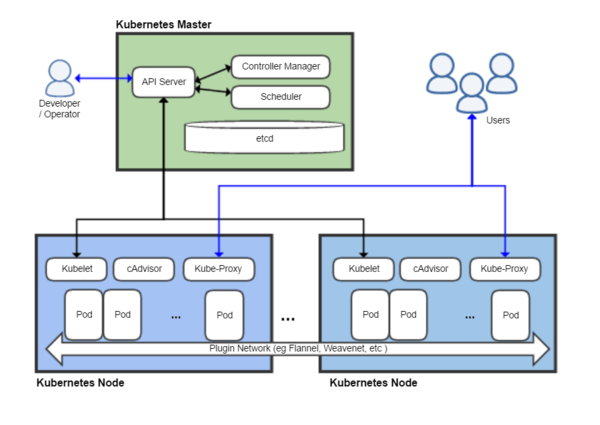
\includegraphics[scale=0.45]{images/Kubernetes.png}
  \caption{Kubernetes architecture diagram \cite{WikiCommons:KubernetesArchitecture}}
\end{figure}


\subsection{Implementation Details}\label{implementation-details}

\subsubsection{Orchestration}\label{orchestration-1}

Given its prominence in the cloud arena and the fact that it is open
source software, we used Kubernetes for orchestration of cloud
components. Having containerized data importers was a requirement from
early on in order to accomplish scalability, and Kubernetes supports the
creation and monitoring of containers natively via its \emph{Pod}
abstraction. Support for Docker containers out-of-the-box was important 
feature for us, as it encapsulated the run-time needs of
our data importers. Since they needed to be scalable, we envisioned from
the beginning that these data importers should be wrapped in some
abstraction which could be launched by some controller or 
orchestrator in our cloud. Docker also gives us the freedom to develop
in any language or technology, so far as the container is well documented
it can be started and called when it is needed. Kuberenetes \emph{Replication Controllers}
then define how many pods or containers need to be running.

In addition, the building blocks of our architecture such
as the queue and the database, which must be guaranteed to be up and
running, were declared as Kubernetes \emph{Services}, which provide
additional self-healing, should these critical components crash.

Additionally, internal DNS provides ease-of-use by being able to refer
to components by a friendly name as opposed to IP addresses. As
mentioned in the Architecture section, scheduling was realized via
simple cron job (see Figure \ref{Kuberenetes-topo}).

Finally, in addition to the command-line interface provided by kops, a
state-of-the-art web interface is provided out-of-the-box, making for a
superior user experience.

\subsubsection{Configuration}\label{configuration}

One of the main advantages of Kubernetes is the ability to specify
behavior of common abstractions via configuration alterable at run-time
rather than by having to program components responsible for carrying out
hard-coded logic. Configuration is provided by YAML files for
registering crons, data importer job runtime configuration, and
service-specific configuration necessary for inter-node communication.


\begin{figure}[htbp]
  \centering
  \hspace*{-0.825 in}
  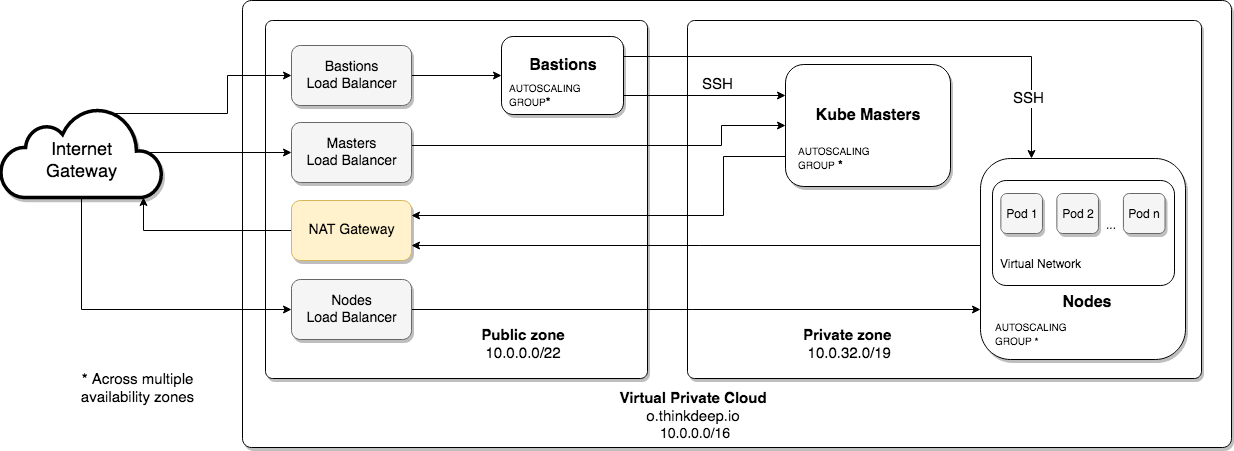
\includegraphics[scale=0.4]{images/Infrastructure_topology.png}
  \caption{Kubernetes Topology}
  \label{Kuberenetes-topo}
\end{figure}


\subsubsection{Deployment Automation}\label{deployment-automation}

Due to the very specific constrains that our project found itself in, a
disproportionately large portion of the effort went into managing
infrastructure. Having no budget meant that whatever infrastructure was
deployed had to be immediately torn down after it was no longer needed.

Difficulties notwithstanding, this meant that the automation process for
deployemnt got well refined, with robust scripts, and the addition of
Kubernetes Operations (kops) and its native support for AWS translated
into an even smoother deployment experience.

Spot instances also played an important role in keeping to the budget,
and support for these were was integrated into the scripts, which
allowed us to monitor and specify the price for spot instances.
